% Options for packages loaded elsewhere
\PassOptionsToPackage{unicode}{hyperref}
\PassOptionsToPackage{hyphens}{url}
\PassOptionsToPackage{dvipsnames,svgnames,x11names}{xcolor}
%
\documentclass[
]{agujournal2019}

\usepackage{amsmath,amssymb}
\usepackage{iftex}
\ifPDFTeX
  \usepackage[T1]{fontenc}
  \usepackage[utf8]{inputenc}
  \usepackage{textcomp} % provide euro and other symbols
\else % if luatex or xetex
  \usepackage{unicode-math}
  \defaultfontfeatures{Scale=MatchLowercase}
  \defaultfontfeatures[\rmfamily]{Ligatures=TeX,Scale=1}
\fi
\usepackage{lmodern}
\ifPDFTeX\else  
    % xetex/luatex font selection
\fi
% Use upquote if available, for straight quotes in verbatim environments
\IfFileExists{upquote.sty}{\usepackage{upquote}}{}
\IfFileExists{microtype.sty}{% use microtype if available
  \usepackage[]{microtype}
  \UseMicrotypeSet[protrusion]{basicmath} % disable protrusion for tt fonts
}{}
\makeatletter
\@ifundefined{KOMAClassName}{% if non-KOMA class
  \IfFileExists{parskip.sty}{%
    \usepackage{parskip}
  }{% else
    \setlength{\parindent}{0pt}
    \setlength{\parskip}{6pt plus 2pt minus 1pt}}
}{% if KOMA class
  \KOMAoptions{parskip=half}}
\makeatother
\usepackage{xcolor}
\setlength{\emergencystretch}{3em} % prevent overfull lines
\setcounter{secnumdepth}{-\maxdimen} % remove section numbering
% Make \paragraph and \subparagraph free-standing
\ifx\paragraph\undefined\else
  \let\oldparagraph\paragraph
  \renewcommand{\paragraph}[1]{\oldparagraph{#1}\mbox{}}
\fi
\ifx\subparagraph\undefined\else
  \let\oldsubparagraph\subparagraph
  \renewcommand{\subparagraph}[1]{\oldsubparagraph{#1}\mbox{}}
\fi


\providecommand{\tightlist}{%
  \setlength{\itemsep}{0pt}\setlength{\parskip}{0pt}}\usepackage{longtable,booktabs,array}
\usepackage{calc} % for calculating minipage widths
% Correct order of tables after \paragraph or \subparagraph
\usepackage{etoolbox}
\makeatletter
\patchcmd\longtable{\par}{\if@noskipsec\mbox{}\fi\par}{}{}
\makeatother
% Allow footnotes in longtable head/foot
\IfFileExists{footnotehyper.sty}{\usepackage{footnotehyper}}{\usepackage{footnote}}
\makesavenoteenv{longtable}
\usepackage{graphicx}
\makeatletter
\def\maxwidth{\ifdim\Gin@nat@width>\linewidth\linewidth\else\Gin@nat@width\fi}
\def\maxheight{\ifdim\Gin@nat@height>\textheight\textheight\else\Gin@nat@height\fi}
\makeatother
% Scale images if necessary, so that they will not overflow the page
% margins by default, and it is still possible to overwrite the defaults
% using explicit options in \includegraphics[width, height, ...]{}
\setkeys{Gin}{width=\maxwidth,height=\maxheight,keepaspectratio}
% Set default figure placement to htbp
\makeatletter
\def\fps@figure{htbp}
\makeatother
% definitions for citeproc citations
\NewDocumentCommand\citeproctext{}{}
\NewDocumentCommand\citeproc{mm}{%
  \begingroup\def\citeproctext{#2}\cite{#1}\endgroup}
\makeatletter
 % allow citations to break across lines
 \let\@cite@ofmt\@firstofone
 % avoid brackets around text for \cite:
 \def\@biblabel#1{}
 \def\@cite#1#2{{#1\if@tempswa , #2\fi}}
\makeatother
\newlength{\cslhangindent}
\setlength{\cslhangindent}{1.5em}
\newlength{\csllabelwidth}
\setlength{\csllabelwidth}{3em}
\newenvironment{CSLReferences}[2] % #1 hanging-indent, #2 entry-spacing
 {\begin{list}{}{%
  \setlength{\itemindent}{0pt}
  \setlength{\leftmargin}{0pt}
  \setlength{\parsep}{0pt}
  % turn on hanging indent if param 1 is 1
  \ifodd #1
   \setlength{\leftmargin}{\cslhangindent}
   \setlength{\itemindent}{-1\cslhangindent}
  \fi
  % set entry spacing
  \setlength{\itemsep}{#2\baselineskip}}}
 {\end{list}}
\usepackage{calc}
\newcommand{\CSLBlock}[1]{\hfill\break\parbox[t]{\linewidth}{\strut\ignorespaces#1\strut}}
\newcommand{\CSLLeftMargin}[1]{\parbox[t]{\csllabelwidth}{\strut#1\strut}}
\newcommand{\CSLRightInline}[1]{\parbox[t]{\linewidth - \csllabelwidth}{\strut#1\strut}}
\newcommand{\CSLIndent}[1]{\hspace{\cslhangindent}#1}

\usepackage{url} %this package should fix any errors with URLs in refs.
\usepackage{lineno}
\usepackage[inline]{trackchanges} %for better track changes. finalnew option will compile document with changes incorporated.
\usepackage{soul}
\linenumbers
\makeatletter
\@ifpackageloaded{caption}{}{\usepackage{caption}}
\AtBeginDocument{%
\ifdefined\contentsname
  \renewcommand*\contentsname{Table of contents}
\else
  \newcommand\contentsname{Table of contents}
\fi
\ifdefined\listfigurename
  \renewcommand*\listfigurename{List of Figures}
\else
  \newcommand\listfigurename{List of Figures}
\fi
\ifdefined\listtablename
  \renewcommand*\listtablename{List of Tables}
\else
  \newcommand\listtablename{List of Tables}
\fi
\ifdefined\figurename
  \renewcommand*\figurename{Figure}
\else
  \newcommand\figurename{Figure}
\fi
\ifdefined\tablename
  \renewcommand*\tablename{Table}
\else
  \newcommand\tablename{Table}
\fi
}
\@ifpackageloaded{float}{}{\usepackage{float}}
\floatstyle{ruled}
\@ifundefined{c@chapter}{\newfloat{codelisting}{h}{lop}}{\newfloat{codelisting}{h}{lop}[chapter]}
\floatname{codelisting}{Listing}
\newcommand*\listoflistings{\listof{codelisting}{List of Listings}}
\makeatother
\makeatletter
\makeatother
\makeatletter
\@ifpackageloaded{caption}{}{\usepackage{caption}}
\@ifpackageloaded{subcaption}{}{\usepackage{subcaption}}
\makeatother
\ifLuaTeX
  \usepackage{selnolig}  % disable illegal ligatures
\fi
\usepackage{bookmark}

\IfFileExists{xurl.sty}{\usepackage{xurl}}{} % add URL line breaks if available
\urlstyle{same} % disable monospaced font for URLs
\hypersetup{
  pdftitle={A Super Cool Study},
  pdfauthor={Josephine Student; John J. Curtin},
  pdfkeywords={Substance use disorders, Precision mental health},
  colorlinks=true,
  linkcolor={blue},
  filecolor={Maroon},
  citecolor={Blue},
  urlcolor={Blue},
  pdfcreator={LaTeX via pandoc}}

\journalname{Journal of Important Findings}

\draftfalse

\begin{document}
\title{A Super Cool Study}

\authors{Josephine Student\affil{1}, John J. Curtin\affil{1}}
\affiliation{1}{Department of Psychology, University of
Wisconsin-Madison, }
\correspondingauthor{John J. Curtin}{jjcurtin@wisc.edu}


\begin{abstract}
This study found some pretty cool results that have both high impact and
important clinical implications. For example \ldots{}
\end{abstract}

\section*{Plain Language Summary}
The ARC produces some of the best science around! \ldots{}



\subsection{Introduction}\label{sec-intro}

You can write your text using markdown.

Top level section headings use \#\#

Notice use of curly braces to label a section if you want to later
cross-reference to it. \#sec- is required as part of the label

\subsubsection{Sub-heading Demo}\label{sub-heading-demo}

You can use sub-headings in your paper as well

\subsubsection{Symbols and Equations}\label{symbols-and-equations}

You can use quarto inline or display math equations as needed. Quarto
provides
\href{https://quarto.org/docs/authoring/markdown-basics.html\#equations}{details}
on the use of these equations.

For example \(x\) and \(y\) are two variables. And here is an important
formula:

\[
p(x) = \frac{e^{-\lambda} \lambda^{x}}{x !}
\]

\subsubsection{Tables}\label{tables}

Tables are generally created and output from notebooks in the /notebooks
folder. You can then embed these tables in your manuscript.

\phantomsection\label{table-1}
\begin{longtable}[]{@{}
  >{\raggedright\arraybackslash}p{(\columnwidth - 10\tabcolsep) * \real{0.1667}}
  >{\raggedleft\arraybackslash}p{(\columnwidth - 10\tabcolsep) * \real{0.1667}}
  >{\raggedleft\arraybackslash}p{(\columnwidth - 10\tabcolsep) * \real{0.1667}}
  >{\raggedleft\arraybackslash}p{(\columnwidth - 10\tabcolsep) * \real{0.1667}}
  >{\raggedleft\arraybackslash}p{(\columnwidth - 10\tabcolsep) * \real{0.1667}}
  >{\raggedleft\arraybackslash}p{(\columnwidth - 10\tabcolsep) * \real{0.1667}}@{}}
\caption{Table 1. A table.}\tabularnewline
\toprule\noalign{}
\begin{minipage}[b]{\linewidth}\raggedright
\end{minipage} &
\multicolumn{2}{>{\centering\arraybackslash}p{(\columnwidth - 10\tabcolsep) * \real{0.3333} + 2\tabcolsep}}{%
\begin{minipage}[b]{\linewidth}\centering
Group 1
\end{minipage}} &
\multicolumn{2}{>{\centering\arraybackslash}p{(\columnwidth - 10\tabcolsep) * \real{0.3333} + 2\tabcolsep}}{%
\begin{minipage}[b]{\linewidth}\centering
Group 2
\end{minipage}} & \begin{minipage}[b]{\linewidth}\centering
Group 3
\end{minipage} \\
\begin{minipage}[b]{\linewidth}\raggedright
\end{minipage} & \begin{minipage}[b]{\linewidth}\raggedleft
mpg
\end{minipage} & \begin{minipage}[b]{\linewidth}\raggedleft
cyl
\end{minipage} & \begin{minipage}[b]{\linewidth}\raggedleft
disp
\end{minipage} & \begin{minipage}[b]{\linewidth}\raggedleft
hp
\end{minipage} & \begin{minipage}[b]{\linewidth}\raggedleft
drat
\end{minipage} \\
\midrule\noalign{}
\endfirsthead
\toprule\noalign{}
\begin{minipage}[b]{\linewidth}\raggedright
\end{minipage} &
\multicolumn{2}{>{\centering\arraybackslash}p{(\columnwidth - 10\tabcolsep) * \real{0.3333} + 2\tabcolsep}}{%
\begin{minipage}[b]{\linewidth}\centering
Group 1
\end{minipage}} &
\multicolumn{2}{>{\centering\arraybackslash}p{(\columnwidth - 10\tabcolsep) * \real{0.3333} + 2\tabcolsep}}{%
\begin{minipage}[b]{\linewidth}\centering
Group 2
\end{minipage}} & \begin{minipage}[b]{\linewidth}\centering
Group 3
\end{minipage} \\
\begin{minipage}[b]{\linewidth}\raggedright
\end{minipage} & \begin{minipage}[b]{\linewidth}\raggedleft
mpg
\end{minipage} & \begin{minipage}[b]{\linewidth}\raggedleft
cyl
\end{minipage} & \begin{minipage}[b]{\linewidth}\raggedleft
disp
\end{minipage} & \begin{minipage}[b]{\linewidth}\raggedleft
hp
\end{minipage} & \begin{minipage}[b]{\linewidth}\raggedleft
drat
\end{minipage} \\
\midrule\noalign{}
\endhead
\bottomrule\noalign{}
\endlastfoot
Mazda RX4 & 21.0 & 6 & 160.0 & 110 & 3.90 \\
Mazda RX4 Wag & 21.0 & 6 & 160.0 & 110 & 3.90 \\
Datsun 710 & 22.8 & 4 & 108.0 & 93 & 3.85 \\
Hornet 4 Drive & 21.4 & 6 & 258.0 & 110 & 3.08 \\
Hornet Sportabout & 18.7 & 8 & 360.0 & 175 & 3.15 \\
Valiant & 18.1 & 6 & 225.0 & 105 & 2.76 \\
Duster 360 & 14.3 & 8 & 360.0 & 245 & 3.21 \\
Merc 240D & 24.4 & 4 & 146.7 & 62 & 3.69 \\
Merc 230 & 22.8 & 4 & 140.8 & 95 & 3.92 \\
Merc 280 & 19.2 & 6 & 167.6 & 123 & 3.92 \\
\end{longtable}

Alternatively, this is an example of a simple table that is hard-coded
using markdown table format. We don't recommend this for tables built
from data. Tables values should come directly from data so they don't
need to be typed in and will update if your data change. However, you
may have other uses for simple tables where this method is helpful.

\begin{longtable}[]{@{}ll@{}}
\caption{Recent historic eruptions on La
Palma}\label{tbl-history}\tabularnewline
\toprule\noalign{}
Name & Year \\
\midrule\noalign{}
\endfirsthead
\toprule\noalign{}
Name & Year \\
\midrule\noalign{}
\endhead
\bottomrule\noalign{}
\endlastfoot
Current & 2021 \\
Teneguía & 1971 \\
Nambroque & 1949 \\
El Charco & 1712 \\
Volcán San Antonio & 1677 \\
Volcán San Martin & 1646 \\
Tajuya near El Paso & 1585 \\
Montaña Quemada & 1492 \\
\end{longtable}

\subsubsection{Figures}\label{figures}

Figures are also generally created in separate notebooks and embedded
into your manuscript.

\begin{figure}[H]

\centering{

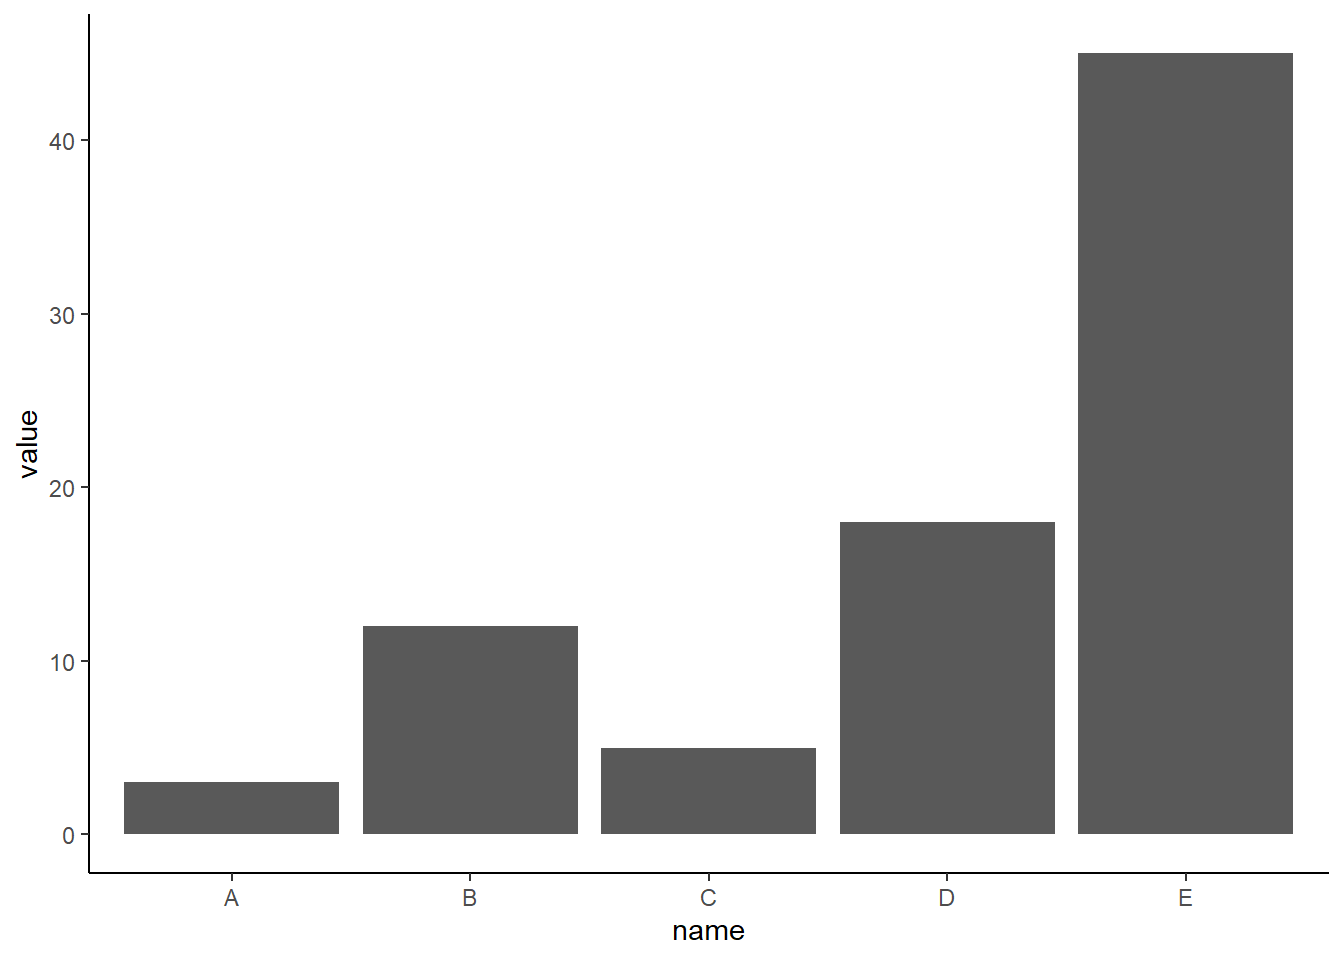
\includegraphics{index_files/figure-latex/notebooks-fig1-fig-1-output-1.png}

}

\caption{\label{fig-1}A Basic Barplot Figure}

\end{figure}%

We can also insert image files directly into our manuscript using images
that are saved in the /images folder

\begin{figure}

\centering{

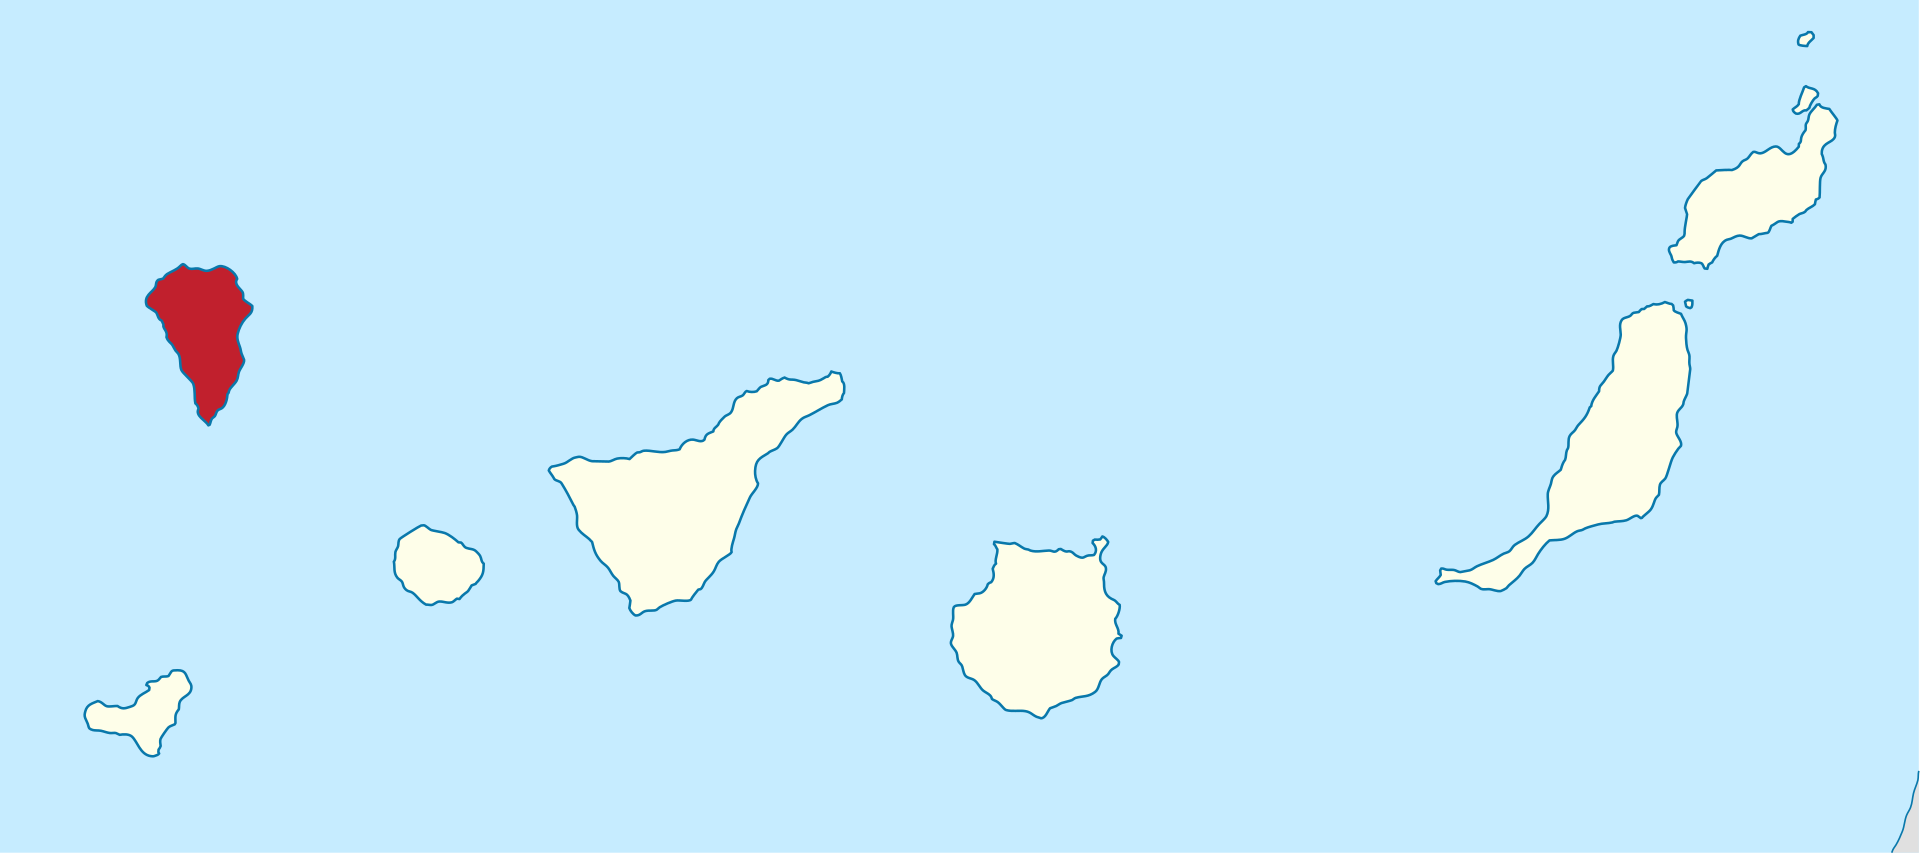
\includegraphics{images/la-palma-map.png}

}

\caption{\label{fig-map}Map of La Palma}

\end{figure}%

\subsubsection{References}\label{references}

We can use cite relevant research in multiple formats. The two most
common are:

\begin{itemize}
\tightlist
\item
  Marrero et al. (2019) concluded something.\\
\item
  These are the conclusions(Marrero et al., 2019).
\end{itemize}

Article references are stored in a .bib file using betterbibtex (BBT)
format. We create these references in Zotero collections.

Although we don't do this regularly I think, if needed you can

\begin{itemize}
\tightlist
\item
  reference other sections in the paper (e.g., Methods are described in
  Section~\ref{sec-methods})
\item
  reference figures elsewhere using the @ symbol. Here is a reference to
  Figure~\ref{fig-1}
\end{itemize}

\subsection{Methods}\label{sec-methods}

\subsection{Results}\label{sec-results}

To add results that are not figures or tables, you will need to open the
analysis objects you saved from these analyses. See lm.qmd as an
example. Generally you will open csv files that contain tidied results.
For example

A significant effect of speed was observed (\(\beta\) = 3.9, t = 9.46, p
= 0.000).

NOTES:

\begin{itemize}
\tightlist
\item
  We should write a function that works with tidied coeffs tables and
  takes the row, column, and number of decimal places to make this code
  simpler.
\item
  This table doesnt contain df. Need to add that to table when saving in
  lm
\end{itemize}

\subsection{Discussion}\label{sec-discussion}

\subsection*{References}\label{references-1}
\addcontentsline{toc}{subsection}{References}

\phantomsection\label{refs}
\begin{CSLReferences}{1}{0}
\vspace{1em}

\bibitem[\citeproctext]{ref-marrero2019}
Marrero, J., García, A., Berrocoso, M., Llinares, Á., Rodríguez-Losada,
A., \& Ortiz, R. (2019). Strategies for the development of volcanic
hazard maps in monogenetic volcanic fields: The example of {La} {Palma}
({Canary} {Islands}). \emph{Journal of Applied Volcanology}, \emph{8}.
\url{https://doi.org/10.1186/s13617-019-0085-5}

\end{CSLReferences}



\end{document}
